\chapter{Algorytm - poszczególne składowe oraz przykłady zastosowania}
\label{cha:AlgorytmPraktyka}

\section{Typ nawierzchni}
\label{sec:surfaceType}

W celu zadbania o bezpieczeństwo osób, ale również o dobrą kondycję techniczną pojazdów poruszających się po drogach, niezbędne jest uwzględnienie typu nawierzchni. Nie można dopuścić do sytuacji, gdy na nawierzchni składającej się głównie że żwiru, znajdowało się znak ograniczenia prędkości o wysokiej wartości. Wtedy ulec awarii może zarówno zawieszenie, jak również jadące przed nimi pojazdy. Aby zapobiec tego typu problemom, algorytm dzieli typ nawierzchni na kilka rodzajów:

\begin{itemize}
\item kostka brukowa
\item żwir
\item drobny żwir
\item nieutwardzona
\item błotnista
\item płyty betonowe
\item droga gruntowa
\item piasek
\item asfalt
\end{itemize}

Najbardziej problematyczna dla kierowców droga to taka, która pokryta jest żwirem, drobnym żwirem, składająca się z piasku lub jest błotnista. W takich przypadkach ograniczenie prędkości wynosi 10 km/h. Niewiele lepsza nawierzchnia to taka, która wyłożona jest zarówno kostką brukową oraz płytami betonowymi. Dla nich, odpowiednia prędkość wynosi 20 km/h. W przypadku drogi nieutwardzonej oraz gruntowej, ograniczenie prędkości wynosi 30 km/h. Dla asfaltu, ze względu na jego strukturę, ograniczenie prędkości praktycznie nie występuje.

Na Rys. \ref{sec:surfaceTypePhoto} zostały umieszczone ograniczenia prędkości dla dróg, których nawierzchnia pokryta jest materiałem innym niż asfalt. Dla celów demonstracyjnych, został on specjalnie pominięty, ponieważ większość dróg jest nim pokryta, przez co Rys. \ref{sec:surfaceTypePhoto} stałby się mało czytelny. Oczywiście ogólny algorytm uwzględnia asfalt.

\begin{figure}[h]
\caption{Ograniczenia prędkości ze względu na rodzaj nawierzchni.}
\label{sec:surfaceTypePhoto}
\centering
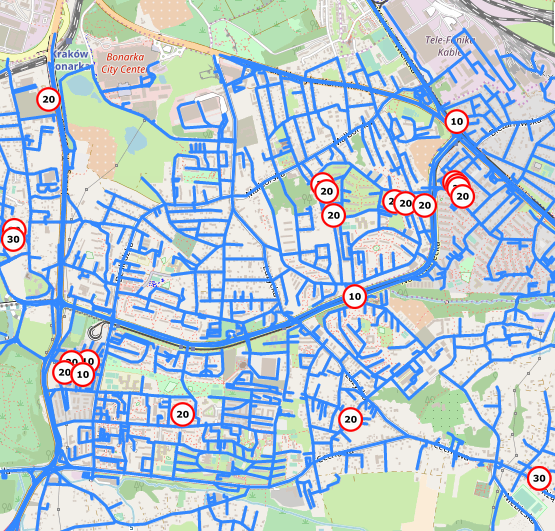
\includegraphics[width=1\textwidth]{surfaceType}
\end{figure}

\newpage
\section{Przejścia dla pieszych}
\label{sec:pedestrialCrossing}
\subsection{Przyporządkowywanie przejść dla pieszych do poszczególnych dróg}

Bardzo ważnym czynnikiem doboru prędkości jest obecność przejść dla pieszych. Te z sygnalizacją świetlną nie stanowią problemu, ponieważ ruch pieszych poruszających się na nich jest ograniczony tylko do sytuacji, gdy sygnalizacja świeci się na zielono. W przypadku przejść bez sygnalizacji, sprawa się komplikuje, ponieważ kierowca jest zobowiązany do zachowania szczególnej ostrożności i zmniejszenia prędkości od 30 km/h.

Do przyporządkowania przejść dla pieszych, do poszczególnych dróg, został wykorzystany wzór \ref{eq:distancePointLineal} na odległość punktu od prostej, przedstawionym w sekcji \ref{sec:ObiektyPunktDrogi}.


Rezultatem wdrożenia powyższego wzoru do programu, są:
\begin{itemize}
\item na niebiesko zaznaczone drogi, na których znajdują się przejścia dla pieszych
\item znakiem ''D-6'' zostały oznaczone przejścia dla pieszych
\end{itemize}
Wynik został przedstawiony na Rys. \ref{sec:PrzejscieDrogi}:

\begin{figure}[h]
\caption{Drogi na których znajdują się przejścia dla pieszych.}
\label{sec:PrzejscieDrogi}
\centering
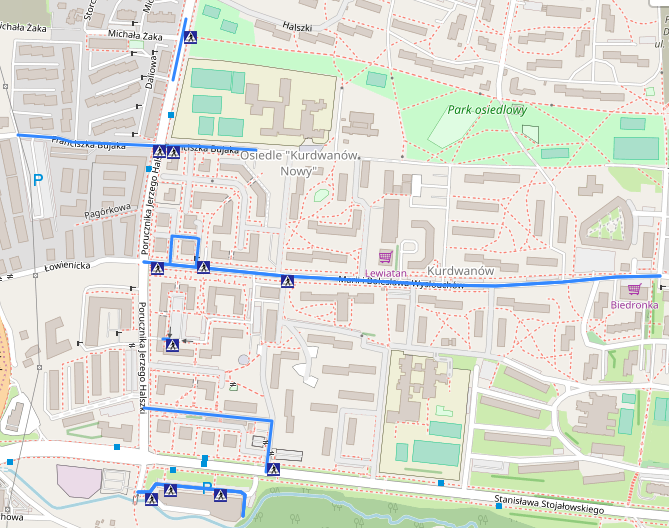
\includegraphics[width=0.9\textwidth]{PrzejscieDrogi}
\end{figure}

Dzięki tak zobrazowanej sytuacji, można ocenić skuteczność algorytmu przyporządkowującemu przejścia dla pieszych do określonych dróg.

\subsection{Wyznaczanie prędkości i umieszczanie jej w odpowiednim miejscu na mapie}

Bezpieczna prędkość w pobliżu nie oznakowanych przejść dla pieszych wynosi ok. 30 km/h. Zapewnia ona zarówno wystarczający czas reakcji, odpowiednio krótką drogę hamowania oraz zmniejsza ryzyko wystąpień potrąceń pieszych.

Algorytm umieszcza znaki ograniczenia prędkości:
\begin{itemize}
\item w przypadku gdy maksymalna prędkość na drodze jest mniejsza bądź równo 30 km/h, nie ma sensu wstawiać znaku
\item w odległości 50 m od przejścia, gdy maksymalna prędkość na drodze jest mniejsza bądź równa 60 km/h
\item w odległości 150 m od przejścia, gdy maksymalna prędkość przekracza 60 km/h
\item w przypadku, gdy przejście dla pieszych znajduje się w odległości mniejszej niż 50m lub 150m (w zależności od maksymalnej prędkości), znak zostanie umieszczony na początku drogi
\item bezpośrednio za przejściem zostanie ustawiony znak przywracającą poprzednie ograniczenie prędkości, za wyjątkiem sytuacji, gdy droga za przejściem dla pieszych jest krótsza niż 100m. W takim wypadku, nie ma sensu zmieniać prędkości.
\end{itemize}

\begin{figure}[h]
\caption{Ograniczenia prędkości przy przejściach dla pieszych.}
\label{sec:przejsciePredkosci}
\centering
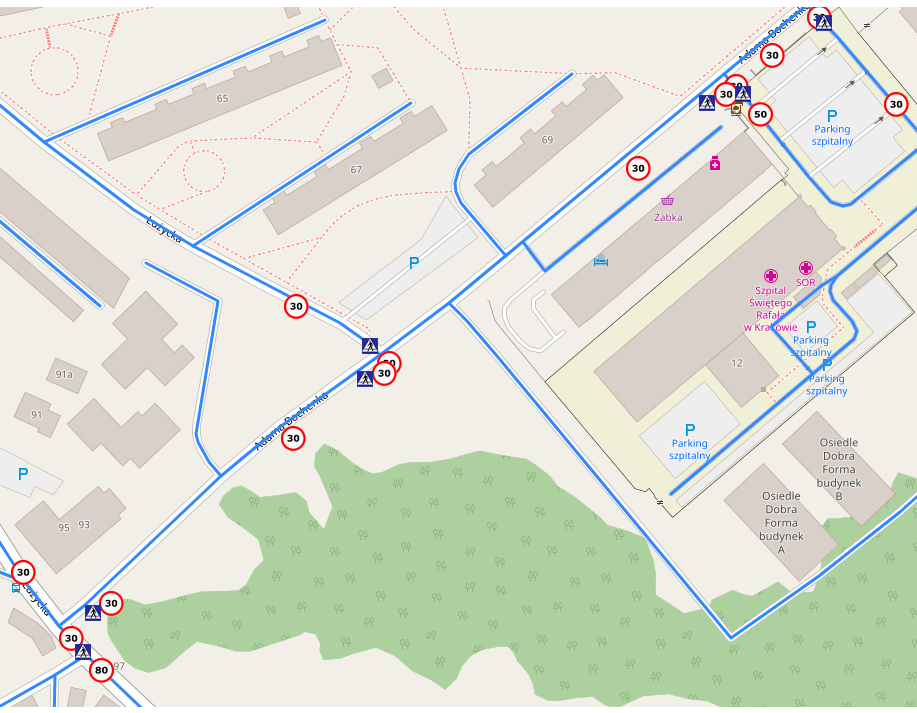
\includegraphics[width=0.8\textwidth]{pedestrian_speed}
\end{figure}

\newpage
\section{Przystanki autobusowe i tramwajowe}
\label{sec:busStopsMain}
Kolejnymi obiektami, uwzględnionymi przez algorytm są przystanki autobusowe i tramwajowe. W ich pobliżu przeważnie znajduje się dość duża grupa ludzi w różnym przedziale wieku. Ponadto zdarzają się sytuacje, że piesi wbiegają na drogę w celu zdążenia na komunikację miejską. Ze względu na takie zachowanie, algorytm ogranicza prędkość przy przystankach autobusowych i tramwajowych do 30 km/h.

Na rys. \ref{sec:busStopBorder} zostały przedstawione przystanki autobusowe i tramwajowe. Wokół nich znajdują się powiększone o 5 metrów obszary pokrywający te obiekty.
\begin{figure}[h]
\caption{Ograniczenie prędkości przed i za światłami drogowymi}
\label{sec:busStopBorder}
\centering
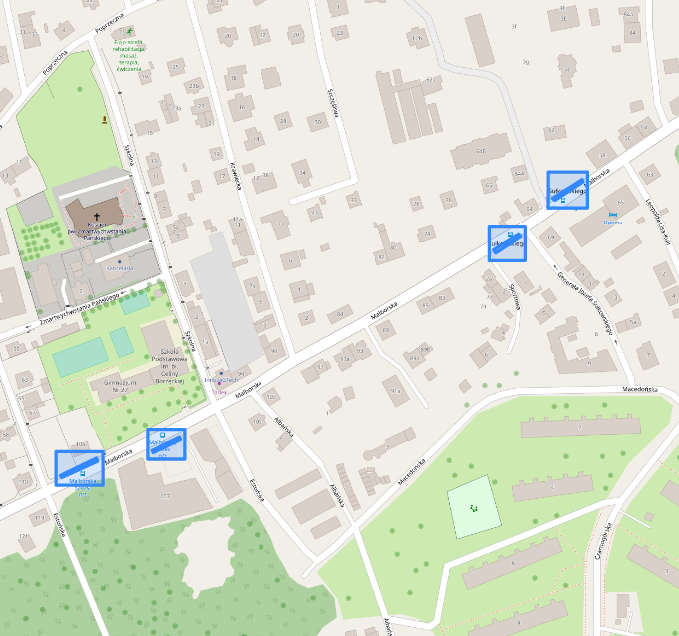
\includegraphics[width=0.9\textwidth]{busStopBorder}
\end{figure}


\newpage
\subsection{Wyznaczanie prędkości i umieszczanie jej w odpowiednim miejscu na mapie}

Najczęściej przystanki autobusowe i tramwajowe znajdują się na drogach o niezbyt wysokiej dopuszczalnej prędkości. W przypadku gdy dopuszczalna prędkość na drodze nie przekracza 30 km/h. nie ma sensu stawiać znaku. W przypadku gdy ograniczenie prędkości na drodze nie przekracza 60 km/h, znak zostanie postawiony w odległości 50 metrów od początku powiększonego obszaru wokół przystanku. Gdy ograniczenie prędkości przekracza 60 km/h, znak zostaje ustawiony w odległości 150 metrów od początku obszaru. 
Znak przywracający poprzednią prędkość, algorytm umieszcza zaraz za obszarem stanowiącym przystanek. Opisana sytuacja została przedstawiona na rys. \ref{sec:busStopSpeed}

\begin{figure}[h]
\caption{Rozmieszczenie znaków w okolicy przystanków autobusowych}
\label{sec:busStopSpeed}
\centering
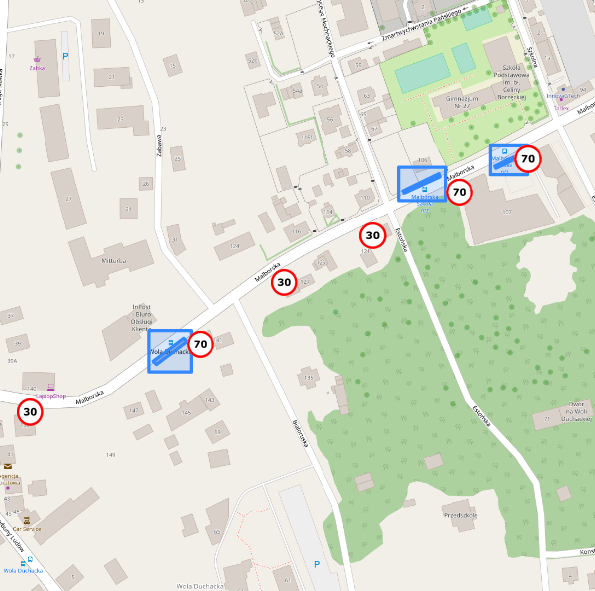
\includegraphics[width=0.9\textwidth]{busStopSpeed}
\end{figure}

\newpage
\section{Przejazdy kolejowe}
\label{sec:railCrossingMain}
\subsection{Przyporządkowywanie przejazdów kolejowych do poszczególnych dróg}

Istotnych parametrem algorytmu wyznaczającego dopuszczalne prędkości jest obecność przejazdów kolejowych. Jak wiadomo, pociąg nie zatrzyma się w miejscu. Jego droga hamowania w głównej mierze zależy od masy oraz prędkości z jaką się porusza. Dla przykładu, pociąg towarowy o masie ok. 1800 ton, jadący z prędkością ok. 50 km/h, zatrzyma się po około 500 m. Dlatego ważne jest określenie prędkości, z jaką samochód może się przemieszczać przed takim przejazdem.

Do przyporządkowania przejazdów kolejowych do poszczególnych dróg, został wykorzystany wzór \ref{eq:distancePointLineal} znajdujący się w rozdziale \ref{sec:pedestrialCrossing}


\begin{figure}[h]
\caption{Drogi na których znajdują się przejazdy kolejowe.}
\label{sec:PrzejazdyKolejowe}
\centering
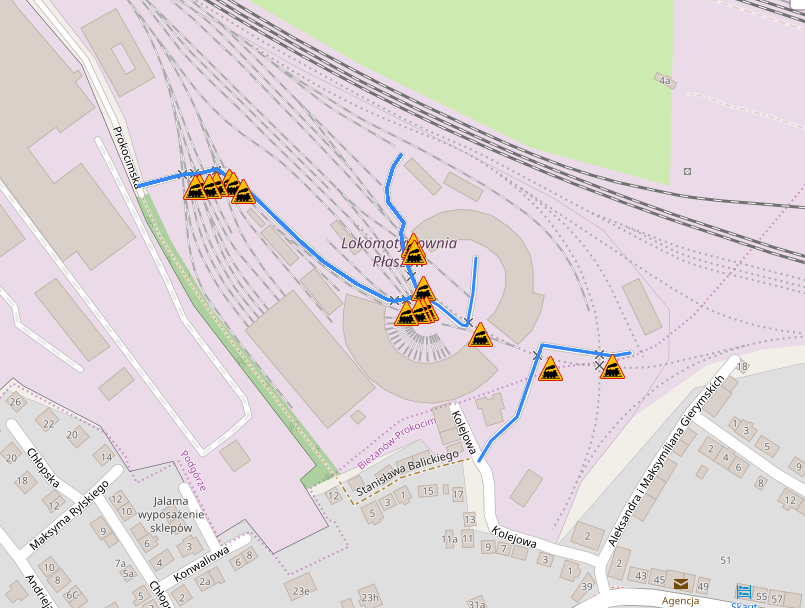
\includegraphics[width=1.0\textwidth]{railCrossing}
\end{figure}

Rys. \ref{sec:PrzejazdyKolejowe} obrazuje wynik przypisania przejazdów kolejowych do poszczególnych dróg:
\begin{itemize}
\item kolorem niebieskim drogi, na których znajdują przejazdy kolejowe
\item znakiem ''A-10'' zostały oznaczone przejazdy kolejowe, pobrane z OpenStreetMap
\end{itemize}

\newpage
\subsection{Wyznaczanie prędkości i umieszczanie jej w odpowiednim miejscu na mapie}

Podobnie jak miało to miejsce w rozdziale \ref{sec:pedestrialCrossing}, umiejscowienie znaków przed przejazdem będzie zależało od kilku czynników:
\begin{itemize}
\item w przypadku gdy maksymalna prędkość na drodze jest mniejsza bądź równo 30 km/h, nie ma sensu wstawiać znaku
\item na  drodze z ograniczeniem prędkości do 60 km/h, znak zostanie umieszczony 50m przed przejazdem kolejowym
\item w przypadku prędkości powyżej 60 km/h, znak zostanie umieszczony w odległości 150m przed przejazdem kolejowym
\item bezpośrednio za przejazdem zostanie ustawiony znak przywracającą poprzednie ograniczenie prędkości, za wyjątkiem sytuacji, gdy droga za przejazdem kolejowym jest krótsza niż 100m. W takim wypadku, nie ma sensu zmieniać prędkości.
\end{itemize}

Rys. \ref{sec:PrzejazdyKolejowe1} obrazuje przejazd kolejowy znajdujący się na dwukierunkowej drodze, na której obowiązuje ograniczenie prędkości do 80 km/h. Dlatego znaki 30 km/h zostały umieszczone 150m przed przejazdem, a zaraz po nim znaki przywracające poprzednią prędkość 80 km/h. Znaki są po obu stronach, gdyż jest do droga dwukierunkowa

\begin{figure}[h]
\caption{Umiejscowienie znaków przed i za przejazdem kolejowym.}
\label{sec:PrzejazdyKolejowe1}
\centering
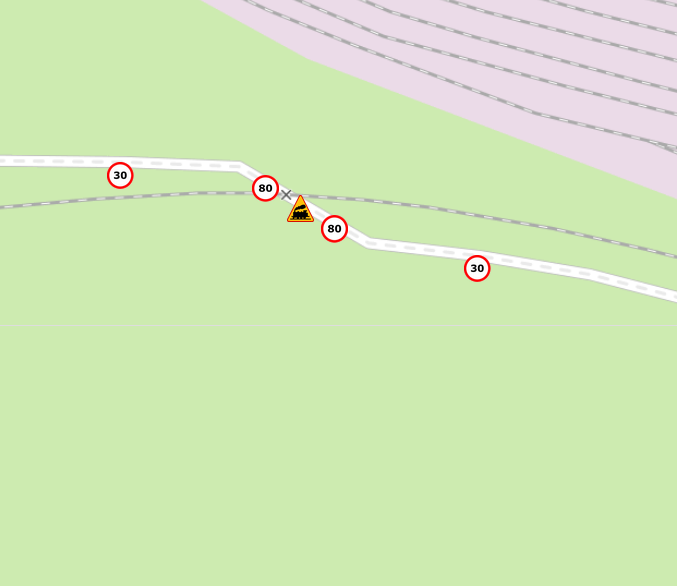
\includegraphics[width=0.7\textwidth]{streetBeforeRail}
\end{figure}


\newpage
\section{Szkoły i miejsca zabaw}
\label{sec:schoolsMain}

Dopuszczalna prędkość, z jaką pojazdy mogą się przemieszczać w pobliżu szkół, placów zabaw lub innych miejsc, przy których mogą znajdować się osoby niepełnoletnie, wynosi 30 km/h. Jest to niezbędne minimum, aby kierowca zdążył zareagować na czas. Na rys. \ref{sec:schoolBorder} po lewej stronie zostało przedstawione przedszkole z placem zabaw przylegającym do niego. Natomiast po prawej znajduje się szkoła podstawowa oraz otoczony wokół niej teren. Jak widać, zostały zaznaczone minimalnym obszarem pokrywającym, powiększonym dodatkowo o 30 metrów z każdej strony

\begin{figure}[h]
\caption{Szkoły i miejsca zabaw}
\label{sec:schoolBorder}
\centering
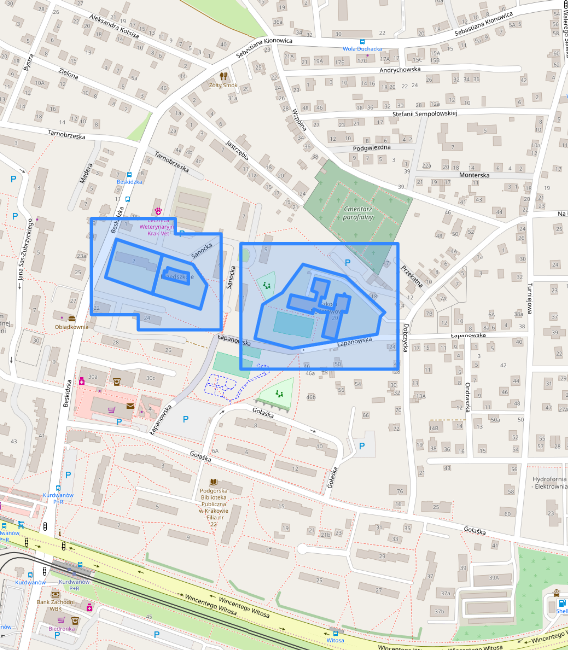
\includegraphics[width=0.9\textwidth]{schoolsBorder}
\end{figure}

\newpage
\subsection{Wyznaczanie prędkości i umieszczanie jej w odpowiednim miejscu na mapie}

Znaki ograniczające dopuszczalną prędkość zostają ustawione w odległości 50 metrów, w przypadku gdy szkoła, znajduje się w pobliżu drogi z ograniczeniem prędkości do 60 km/h. Powyżej tej prędkości znaki zostają umieszczone w odległości 150m. Jest ono umieszczane tylko wtedy, gdy ograniczenie prędkości na drodze jest większe niż 30 km/h. Znak przywracający poprzednie ograniczenia prędkości jest umieszczany bezpośrednio po obszarze w którym znajduje się szkoła. Zostało to przedstawione na rys. \ref{sec:schoolsSpeed}.

\begin{figure}[h]
\caption{Szkoły i miejsca zabaw}
\label{sec:schoolsSpeed}
\centering
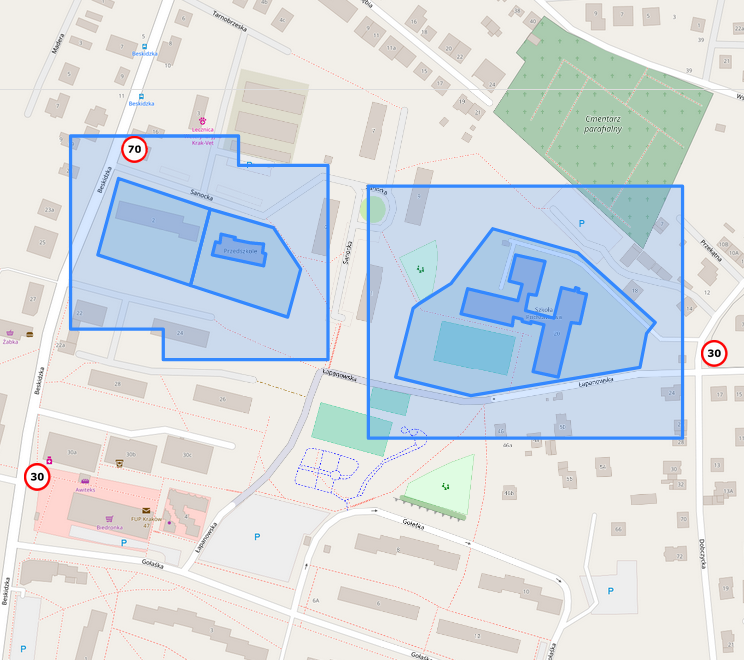
\includegraphics[width=0.95\textwidth]{schoolsSpeed}
\end{figure}


\newpage
\section{Sygnalizacja świetlna}
\label{sec:trafficSignalMain}
\subsection{Przyporządkowywanie sygnalizacji świetlnej do poszczególnych dróg}

Aby kierowca bez problemu mógł zdążyć zareagować na zmieniające się światła sygnalizacji świetlnej, niezbędne jest zredukowanie prędkości do odpowiedniej wartości. Ze względu na fakt iż sygnalizacja widoczna jest z relatywnie dużej odległości, prędkość przed sygnalizacją zostanie ograniczona do ok. 50 km/h.


\begin{figure}[h]
\caption{Drogi na których znajduje się sygnalizacja świetlna.}
\label{sec:PrzejazdyKolejowe2}
\centering
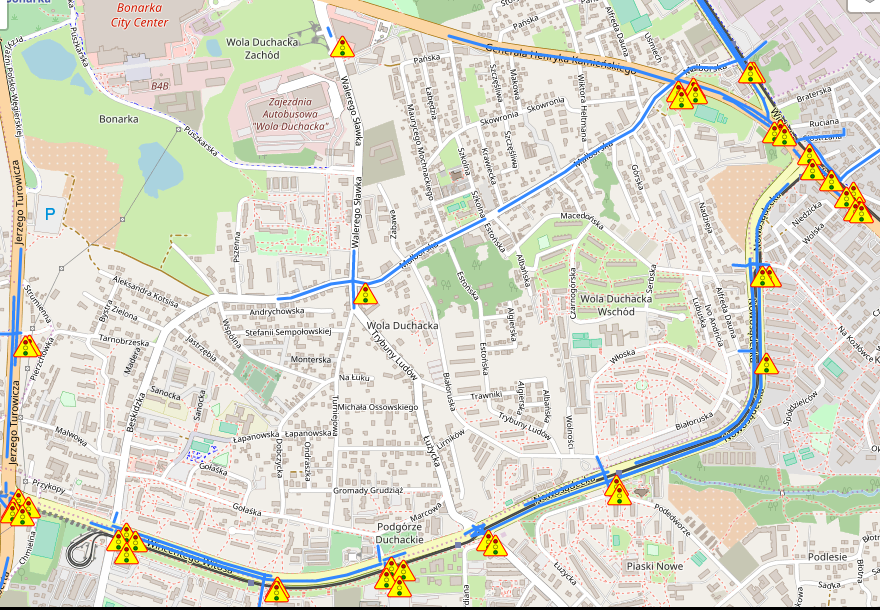
\includegraphics[width=1.1\textwidth]{traffic_sight}
\end{figure}

Rys. \ref{sec:PrzejazdyKolejowe2} ukazuje sposób działania algorytmu przypisującego do drogi sygnalizację świetlną. Zaznaczono na nim:
\begin{itemize}
\item kolorem niebieskim drogi, na których znajduje się sygnalizacja świetlna
\item znakiem ''A-29'' zostały oznaczone sygnalizacje świetlne, pobrane z OpenStreetMap
\end{itemize}

\newpage
\subsection{Wyznaczanie prędkości i umieszczanie jej w odpowiednim miejscu na mapie}

Algorytm umieszcza znaki ograniczenia prędkości w następujący sposób:
\begin{itemize}
\item w przypadku gdy maksymalna prędkość na drodze jest mniejsza bądź równo 50 km/h, nie ma sensu wstawiać znaku
\item 50m przed sygnalizacją na drodze z ograniczeniem prędkości do 60 km/h
\item 150m przed sygnalizacją na drodze z ograniczeniem prędkości powyżej 60 km/h
\item w przypadku drogi dwukierunkowej, zarówno przed, jak i za sygnalizacją
\item bezpośrednio za sygnalizacją zostanie ustawiony znak przywracającą poprzednie ograniczenie prędkości, za wyjątkiem sytuacji, gdy droga za sygnalizacją świetlną jest krótsza niż 100m. W takim wypadku, nie ma sensu zmieniać prędkości.
\end{itemize}


Rys. \ref{sec:znakiSwiatla} obrazuje fragment skrzyżowania na której znajduje się sygnalizacja świetlna. Ograniczenie prędkości na drogach wynosi od 70 do 80 km/h, dlatego algorytm umieścił znak ograniczenia prędkości do 50 km/h, 150m przed sygnalizacją oraz znak przywracający poprzednią prędkość zaraz za sygnalizacją.

\begin{figure}[h]
\caption{Ograniczenie prędkości przed i za światłami drogowymi}
\label{sec:znakiSwiatla}
\centering
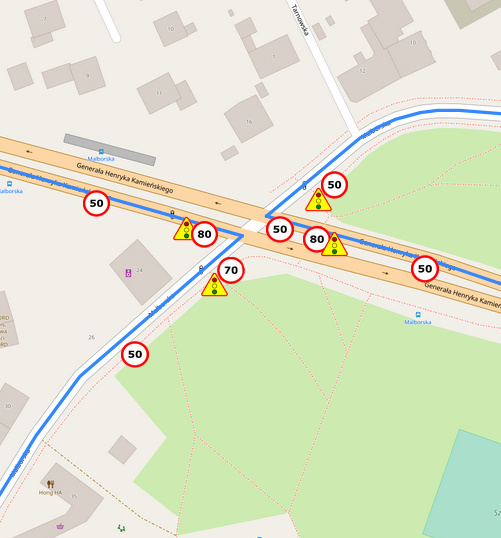
\includegraphics[width=0.65\textwidth]{speedBeforeSignals}
\end{figure}

\newpage
\section{Sklepy i miejsca kultów religijnych}
\label{sec:shoopsChurchesMain}

Zwiększone ruch samochodów oraz pieszych przy sklepach najczęściej zauważalny jest w godzinach wieczornych i w weekendy. Natomiast zwiększenie ruchu w miejscach kultu religijnego widoczne jest w czasie świąt. Z tego powodu, algorytm musi uwzględniać takie miejsca. Zostały one przedstawione na rys. \ref{sec:shopsBorder}.

\begin{figure}[h]
\caption{Szkoły i miejsca religijne}
\label{sec:shopsBorder}
\centering
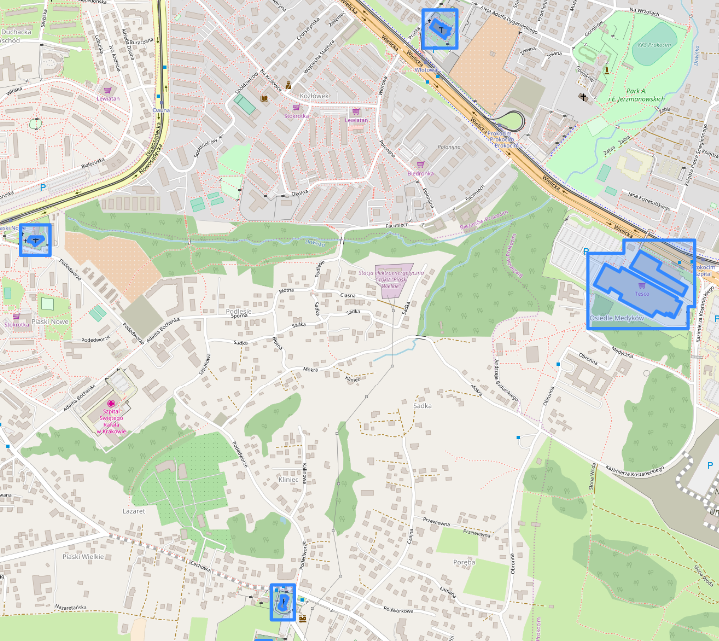
\includegraphics[width=0.9\textwidth]{shopsBorder}
\end{figure}

Na rys. \ref{sec:shopsBorder} widoczne są obramowania kościołów i sklepów. Ponadto otoczone są powiększonym obszarem pokrywającym, reprezentującym strefę ograniczenia prędkości.

\newpage
\subsection{Wyznaczanie prędkości i umieszczanie jej w odpowiednim miejscu na mapie}

Dopuszczalna prędkość z jaką można się poruszać w obrębie sklepów i miejsc kultów wynosi 30 km/h. Znak ograniczenia prędkości ustawiany jest w odległości 50 metrów od początku strefy ograniczonej prędkości, w przypadku gdy dopuszczalna prędkość na drodze nie przekracza 60 km/h. W przeciwnym razie znak ustawiany jest w odległości 150 metrów od początku strefy. Bezpośrednio za końcem strefy ustawiany jest znak przywracający poprzednią prędkość. Sytuacja ta została przedstawiona rys. \ref{sec:shopsSpeed}.

\begin{figure}[h]
\caption{Szkoły i miejsca religijne razem w wyznaczonymi prędkościami}
\label{sec:shopsSpeed}
\centering
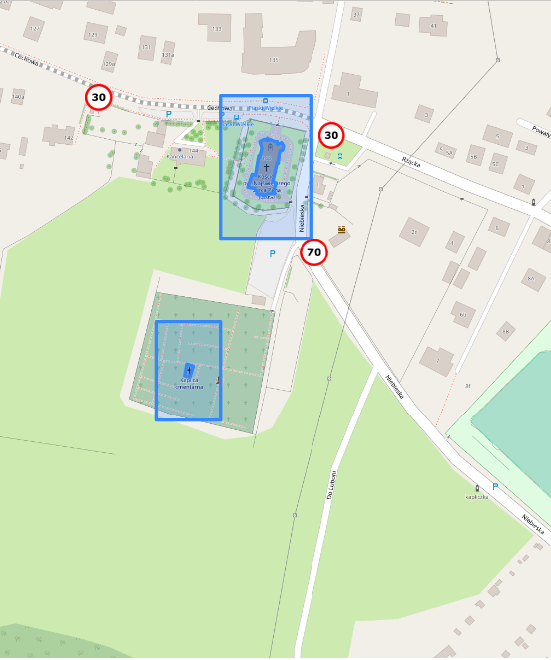
\includegraphics[width=1\textwidth]{shopsSpeed}
\end{figure}
\newpage
\section{Liczba pasów ruchu}
\label{sec:laneNumber}

Maksymalna dozwolona prędkość jest zależna również od liczby pasów ruchu. Im jest ich więcej, tym większą prędkość można rozwijać. Dlatego algorytm zwiększa dopuszczalną prędkość o 10 km/h w przypadku gdy liczba pasów ruchu jest większa niż jeden. Na rys \ref{sec:laneNumber} zostały zaznaczone ulice, których liczba pasów ruchu wynosi przynajmniej 2, oraz prędkości nie uwzględniające pasów ruchu. 

\begin{figure}[h]
\caption{Prędkość przy nieuwzględnieniu liczby pasów ruchu}
\label{sec:laneNumber}
\centering
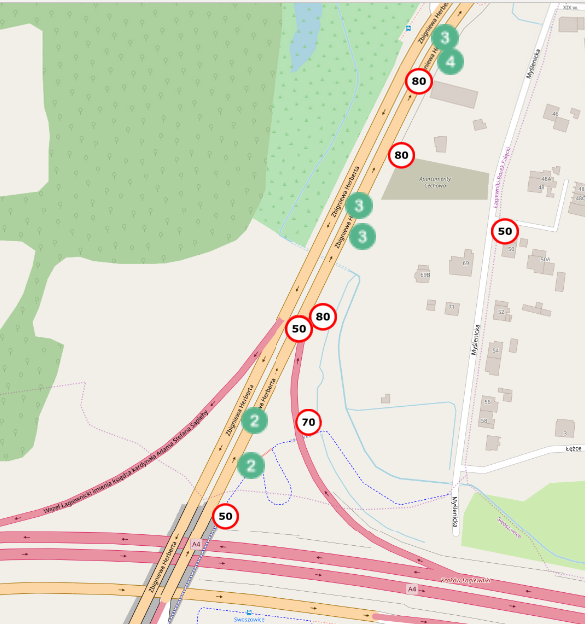
\includegraphics[width=0.95\textwidth]{laneNumber}
\end{figure}

\newpage
Na rys. \ref{sec:laneNumberAfter} zostały przedstawione prędkości już z uwzględnioną liczbą pasów ruchu. Zauważyć można, że tam, gdzie liczba pasów jest większa niż jeden, prędkość została zwiększone, a tam gdzie występuje tylko jeden pas ruchu, prędkość pozostała niezmieniona. Ograniczenie prędkości dotyczy całego odcinka drogi, dlatego znak ograniczenia prędkości jest umieszczany na początku każdej drogi.
\begin{figure}[h]
\caption{Prędkość uwzględniająca liczbę pasów ruchu}
\label{sec:laneNumberAfter}
\centering
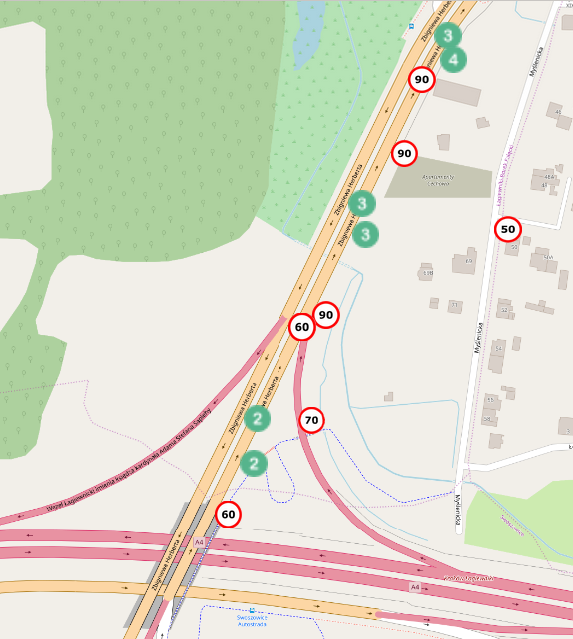
\includegraphics[width=0.95\textwidth]{laneNumberAfter}
\end{figure}

\newpage
\section{Rodzaj drogi}
\label{sec:typeOfRoad}
Algorytm rozróżnia sześć podstawowych typów dróg, w skład których wchodzą:
\begin{itemize}
\item dojazdowe
\item lokalne
\item główne
\item główne przyspieszonego ruchu
\item ekspresowe
\item autostrady
\end{itemize}

Dla dróg dojazdowych i lokalnych ograniczenie prędkość wyznaczone przez algorytm wynosi 30 km/h. Dla dróg głównych ograniczenie prędkości wynosi 70 km/h, dla dróg głównych przyspieszonego ruchu 80 km/h, natomiast dla dróg ekspresowych 120 km/h oraz dla autostrad 140 km/h. Ograniczenia prędkości ze względu na typ drogi zostały przedstawione na rys \ref{sec:typeOfRoad}
\begin{figure}[h]
\caption{Ograniczenie prędkości w zależności od rodzajów dróg}
\label{sec:typeOfRoad}
\centering
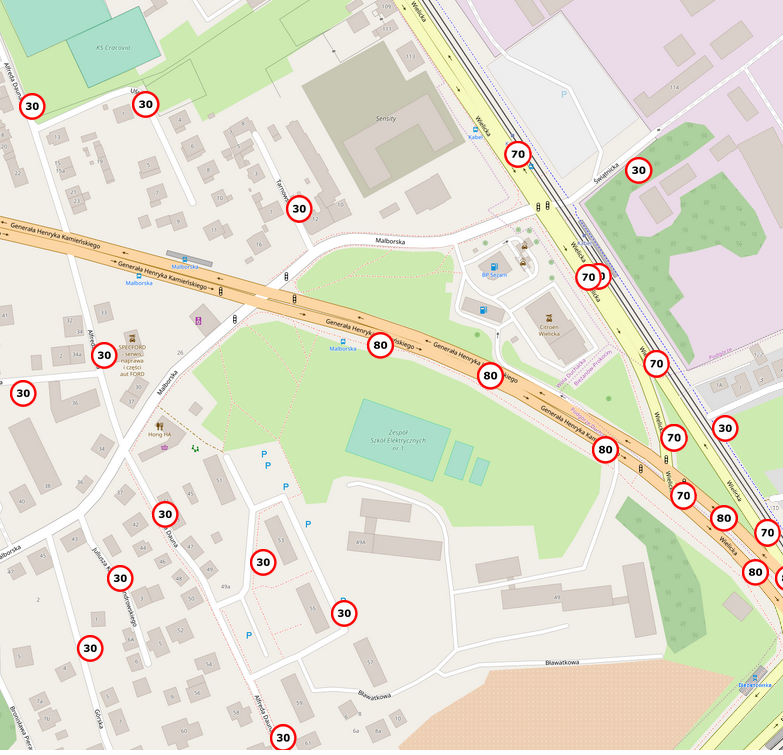
\includegraphics[width=0.7\textwidth]{typeOfRoad}
\end{figure}

\newpage
\section{Zakręty}
\label{sec:zakretyMain}
Ostatnim czynnikiem wpływającym na prędkość wyznaczoną przez algorytm są zakręty. Każdy zakręt posiada wyliczony swój promień skrętu. Dokładny opis ich wyznaczenia został przedstawiony w sekcji \ref{sec:WyznaczaniePromieniaSkrętuDlaZakrętówDanejDrogi}
Na rys. \ref{sec:zakrety} zostały zakręty, dla których promień skrętu jest większy niż 50m
\begin{figure}[h]
\caption{Zaznaczone zakręty}
\label{sec:zakrety}
\centering
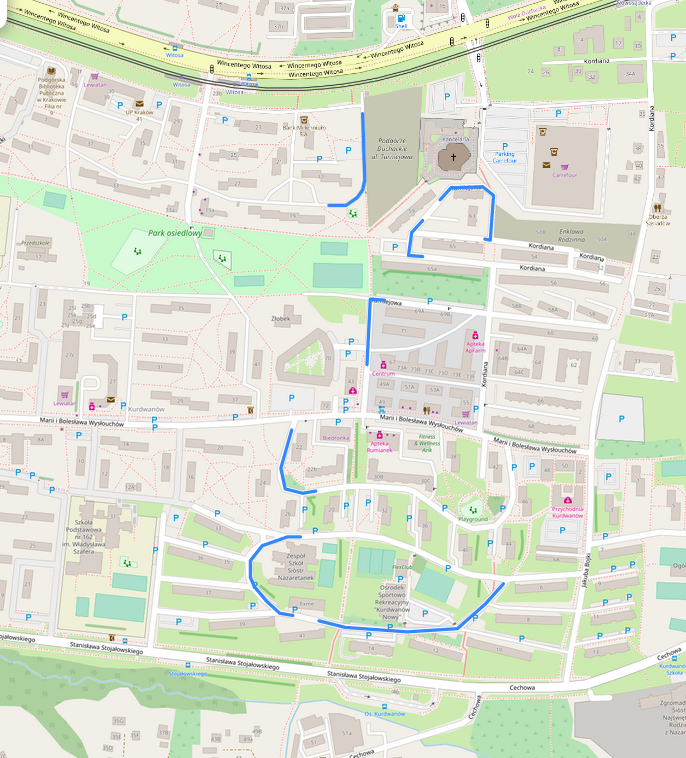
\includegraphics[width=0.9\textwidth]{zakrety}
\end{figure}

\newpage
\subsection{Wyznaczanie prędkości i umieszczanie jej w odpowiednim miejscu na mapie}
Algorytm uwzględnia trzy rodzaje promieni skrętów: 
\begin{itemize}
\item mały promień skrętu o długości promienia nie przekraczającej 300 metrów
\item średni promień skrętu o długości promienia między 300 a 600 metrów
\item duży promień skrętu o długości promienia powyżej 600 metrów.
\end{itemize}
Ograniczenie prędkości w przypadku małego promienia skrętu jest zmniejszane o 10 km/h, w przypadku średniego promienia skrętu, dopuszczalna prędkość zmniejsza się o 20 km/h, natomiast przy dużym promieniu skrętu, prędkość zredukowana jest o 30 km/h. 

Znak ustawiany jest 50 metrów od początku skrętu, w przypadku gdy dopuszczalna prędkość nie przekracza 60 km/h. W przeciwnym wypadku, znak umieszczany jest 150 metrów od początku skrętu. Bezpośrednio na końcu zakrętu, umieszczany jest znak przywracający poprzednią prędkość. Sytuację tą obrazuje rys \ref{sec:zakretySpeed}
\begin{figure}[h]
\caption{Zaznaczone zakręty razem z wyliczonymi prędkościami}
\label{sec:zakretySpeed}
\centering
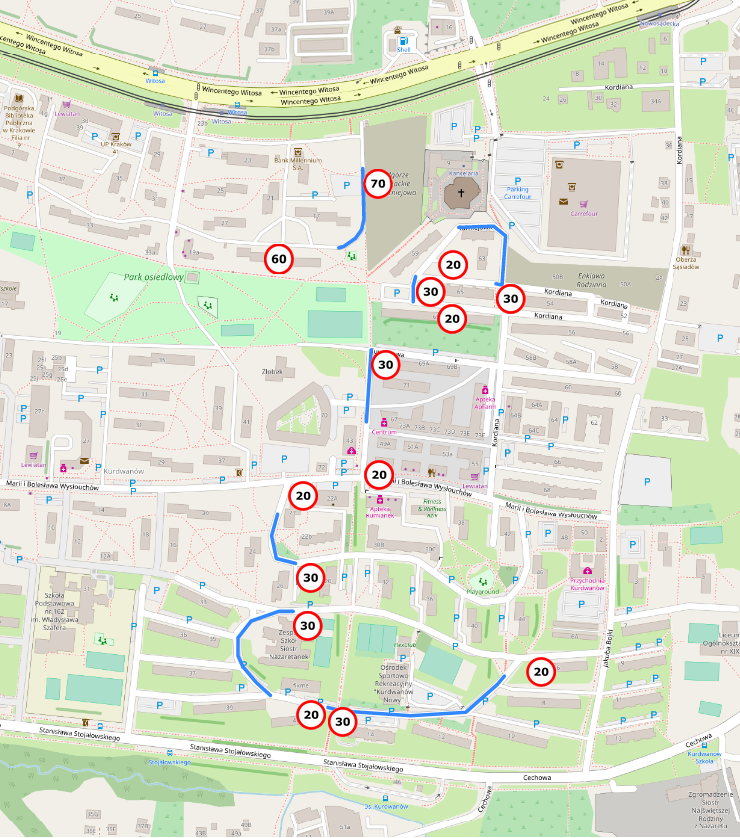
\includegraphics[width=0.7\textwidth]{CurvesSpeed}
\end{figure}

\newpage
\section{Działanie algorytmu}
\label{sec:speedLimitLocalization}



Na początku wyliczane jest domyślne ograniczenie prędkości dla każdej drogi na podstawie poniższych kryteriów:
\begin{itemize}
\item Typ nawierzchni - szczegóły w rozdziale \ref{sec:surfaceType}
\item Rodzaj drogi - szczegóły w rozdziale \ref{sec:typeOfRoad}
\item Długość drogi
\item Liczby pasów ruchu - szczegóły w rozdziale \ref{sec:laneNumber}
\end{itemize}

Następnie algorytm przystępuje do umieszczania znaków na drodze według następującej kolejności:
\begin{itemize}
\item jeśli droga jest krótsza niż 50m, nie ustawia znaku
\item jeśli domyślna prędkość jest mniejsza bądź równa ograniczeniu prędkości wymaganym przez obiekt typu przejście dla pieszych, szkoła, zakręt itp, nie ustawia znaku
\item jeśli droga lub jej fragment znajdują się w strefie ograniczonej prędkości, to wewnątrz tej strefy nie są ustawiane żadne inne ograniczenia prędkości.
\item na początku drogi ustawia znak domyślnego ograniczenia prędkości, chyba że zachodzą następujące czynniki:
\begin{itemize}
\item gdy domyślna prędkości jest mniejsza bądź równa 60 km/h i obiekt typu przejście dla pieszych, szkoła, zakręt itp znajduje się w  odległości mniejszej bądź równej 50m
\item gdy domyślna prędkości przekracza 60 km/h i obiekt znajduje się w  odległości mniejszej bądź równej 150m 
\end{itemize}
w takim przypadku na początku drogi ustawiane jest ograniczenie prędkości dla danego obiektu.
\item w odległości 50 metrów od obiektów jednowymiarowych typu przejście dla pieszych itp, lub 50 metrów przed początkiem strefy ograniczonej prędkości, gdy dopuszczalna prędkość jest mniejsza bądź równa 60 km/h. Dotyczy sytuacji, gdy w odległości nie większej niż 50 metrów przed obiektem, nie znajduje się inny obiekt. W przeciwnym razie, ograniczenie prędkości nie jest ustawiane.
\item w odległości 150 metrów od obiektów jednowymiarowych typu przejście dla pieszych itp, lub 150 metrów przed początkiem strefy ograniczonej prędkości, gdy dopuszczalna prędkość przekracza 60 km/h. Dotyczy sytuacji, gdy w odległości nie większej niż 150 metrów przed obiektem, nie znajduje się inny obiekt. W przeciwnym razie, ograniczenie prędkości nie jest ustawiane.
\item jeśli za obiektem typu przejście dla pieszych lub za strefą ograniczonej prędkości znajduje się inny obiekt ustawiony w odległości:
\begin{itemize}
\item 50 metrów, w przypadku domyślnej prędkości na drodze nie przekraczającej 60 km/h
\item 150 metrów, w przypadku domyślnej prędkości większej niż 60 km/h
\end{itemize}
to bezpośrednio za tym obiektem ustawia znak ograniczenia prędkości wymagany przez następny obiekt. Chyba że ograniczenie prędkości dopuszczalne dla następnego obiektu jest mniejsze bądź równe aktualnemu. W takim przypadku nie ustawia znaku
\item bezpośrednio za obiektem przywracana jest domyślna prędkość na drodze, chyba że 
\begin{itemize}
\item długość drogi za obiektem jest mniejsza niż 50 metrów
\item domyślne ograniczenie prędkości jest mniejsze bądź równe ograniczeniu wymaganemu przed dany obiekt
\end{itemize}
W takich przypadkach nie przywraca domyślnej prędkości.
\item Jeśli koło siebie znajdują się znaki prędkości z takim samym ograniczeniem - algorytm zostawia pierwszy, kolejne usuwa
\end{itemize}



